\problemname{Castle Wall}

\noindent

The owner of the castle Drakfjälls Kastell is worried about a potential siege. If this happens, he wants the wall to be sturdy, 
so he plans to reinforce it. The castle wall consists of $N$ wall segments arranged in a line. Each wall segment has 
a certain height. Below is an example of how the wall might look.

\begin{center}
  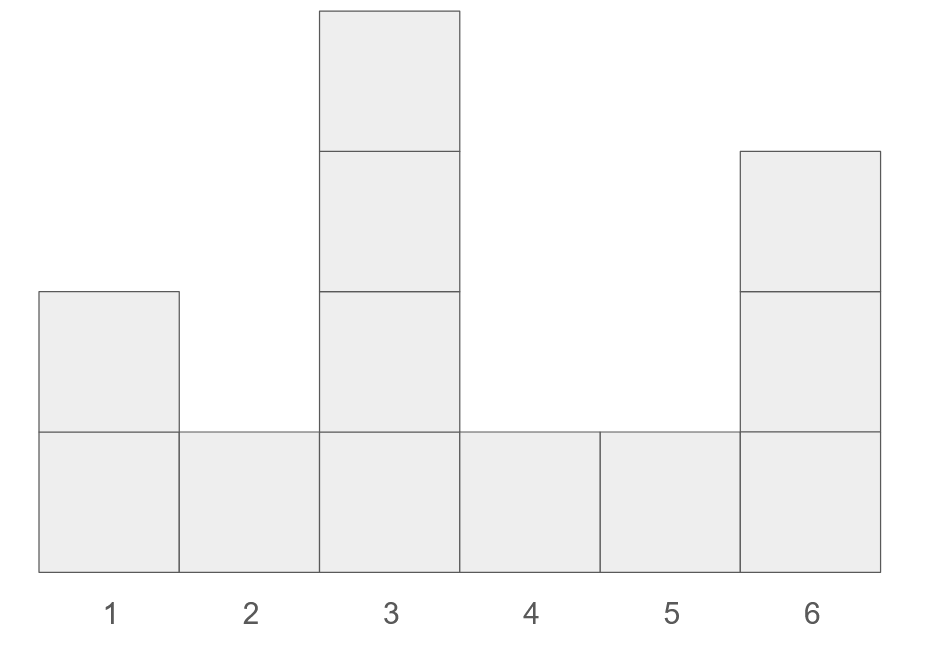
\includegraphics[scale=0.3]{mur1.png}
\end{center}

The castle owner is also concerned about moisture damage when it rains, which could potentially worsen 
if he reinforces the wall. When it rains, all the wall's gaps will fill up with water, as long as the 
water cannot drain off at the sides. If it had rained on the previous example wall, water would have 
collected at the blue squares.

\begin{center}
  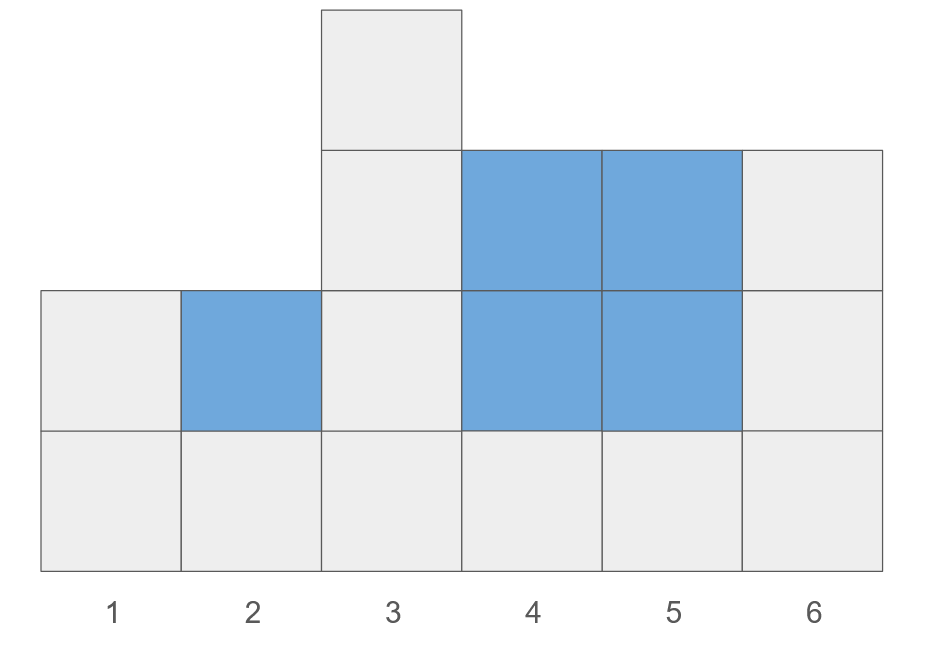
\includegraphics[scale=0.3]{mur2.png}
\end{center}

To be strategic with his reconstruction, he wants to know how certain reinforcements would affect 
the amount of rainwater that collects in the wall if parts of it were destroyed in a siege. 
At his disposal, he has you, the castle's theoretical computer scientist.
The castle owner will ask you two types of queries:
\begin{itemize}
  \item Given two values $l$ and $r$. If all wall segments are destroyed except those in the interval $[l,r]$, 
  how much rainwater would collect in the wall if it starts raining?
  Note that the wall isn't actually destroyed, so this doesn't affect future queries.
  \item Given two values $i$ and $w$, increase the height of the $i$th wall segment by $w$. 
  This is a permanent change that will affect future queries.
\end{itemize}

\section*{Input}
The first line of input contains the integers $N$ and $Q$ ($1 \le N, Q \le 2 \cdot 10^5$),
the number of wall segments and the number of queries.

Then follow $N$ integers $h_1, h_2, \dots, h_N$ ($1 \leq h_i \leq 10^9$), the height of each wall segment.\\

The following $Q$ lines describe all queries. Each query starts with an integer $T$, which is either $1$ or $2$.
\begin{itemize}
  \item If $T=1$, it's followed by $l, r$ ($1 \leq l \leq r \leq N$). You should then output the answer to a type $1$ query as described above.
  \item If $T=2$, it's followed by $i, w$ ($1 \leq i \leq N$, $1 \leq w \leq 10^9$). You should then increase the height of the $i$th wall segment by $w$.
  It's guaranteed that the height of the wall segment remains less than or equal to $10^9$ after this.
\end{itemize}

\section*{Output}
For each type $1$ query, output the amount of water that collects if it starts raining after all wall segments outside
the given interval are destroyed.

\section*{Scoring}
Your solution will be tested on a set of test groups, each worth a number of points. Each test group contains
a set of test cases. To get the points for a test group you need to solve all test cases in the test group.

\noindent
\begin{tabular}{| l | l | p{12cm} |}
  \hline
  \textbf{Group} & \textbf{Points} & \textbf{Constraints} \\ \hline
  $1$    & $13$       & $N, Q \leq 1000$ \\ \hline
  $2$    & $20$       & All queries are of type $1$. \\ \hline
  $3$    & $17$       & $h_i$ and $w$ are chosen uniformly randomly among their valid values \footnote{See https://en.wikipedia.org/wiki/Discrete\_uniform\_distribution}. \\ \hline
  $4$    & $23$       & $N, Q \leq 70000$ \\ \hline
  $5$    & $27$       & No additional constraints. \\ \hline
\end{tabular}

\section*{Explanation of Sample 1}
In the first query, we're asked to calculate the amount of water that collects if we destroy everything outside $[1,6]$. Since
$[1,6]$ constitutes the entire wall, nothing is destroyed.
\begin{center}
  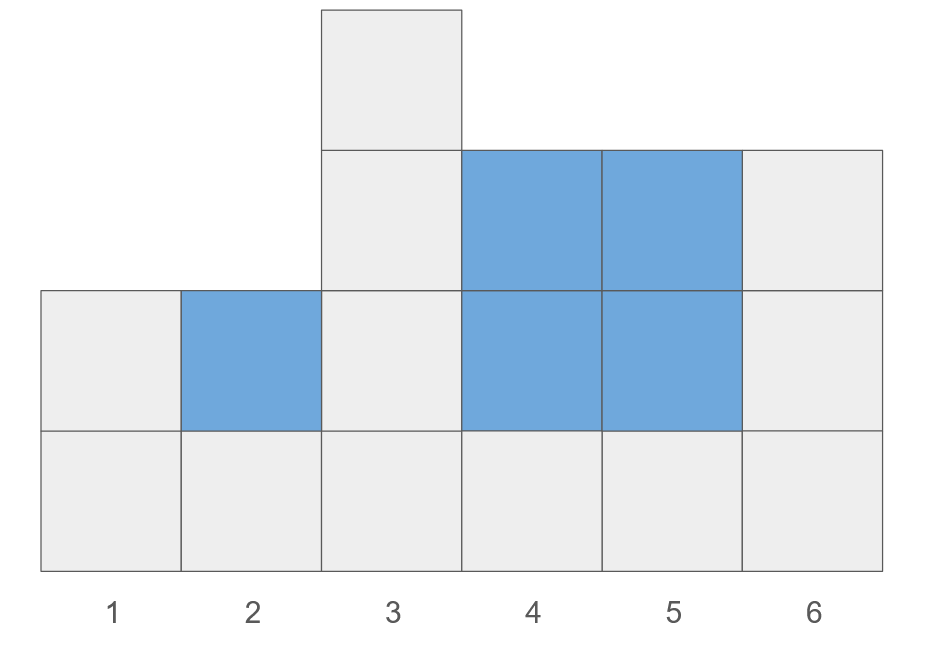
\includegraphics[scale=0.2]{mur2.png}
\end{center}

In the second query, the Castle owner wants to know what happens if part of the right end of the wall is destroyed.
The wall segments that would be destroyed are marked in dark gray.

\begin{center}
  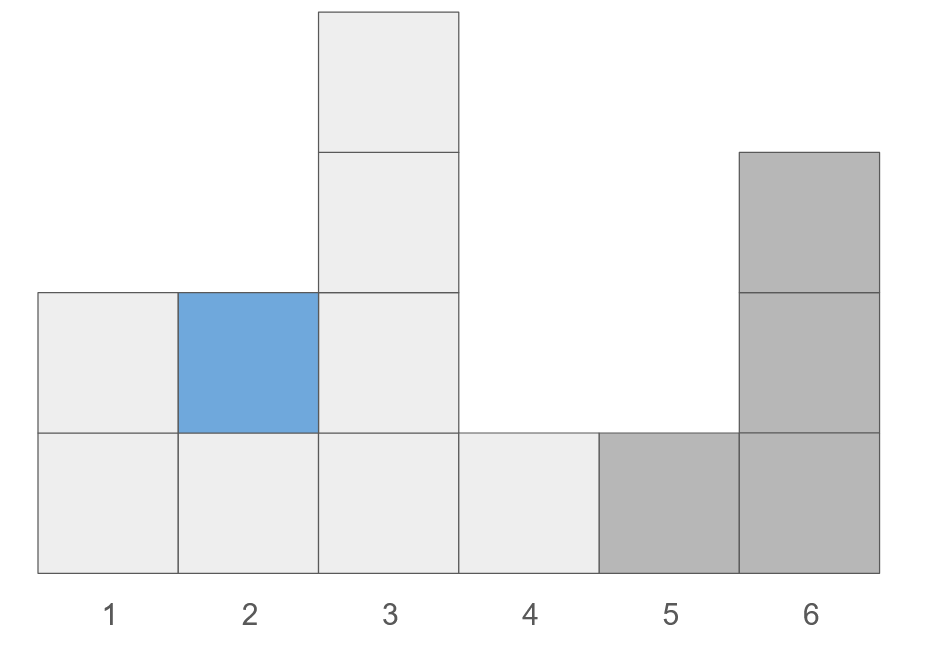
\includegraphics[scale=0.2]{mur3.png}
\end{center}

In the third query, part of the wall is raised. This affects the fourth query, which looks like the following.

\begin{center}
  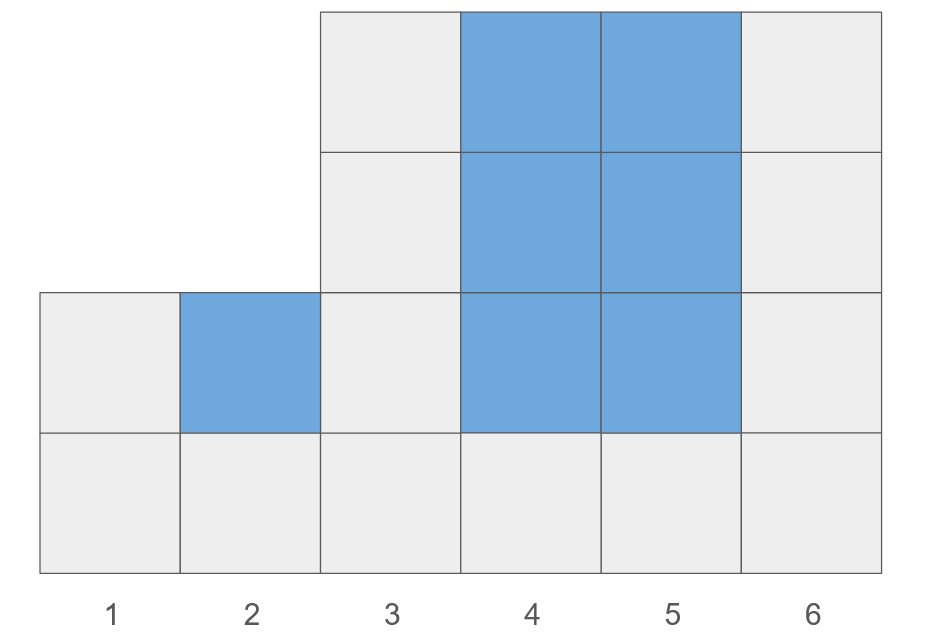
\includegraphics[scale=0.2]{mur4.png}
\end{center} 